
\chapter{Bug/Issue Tracking}
\section{Bugzilla}
Bugzilla ist ein von Terry Weissmann ursprünglich in TCL jetzt in Perl
geschriebenes
Problembehandlungssystem, welches im Open-Source-Umfeld einen
Defacto-Standard darstellt.
\begin{center}

\includegraphics[width=0.18\linewidth]{config-management/buggie}\hfill
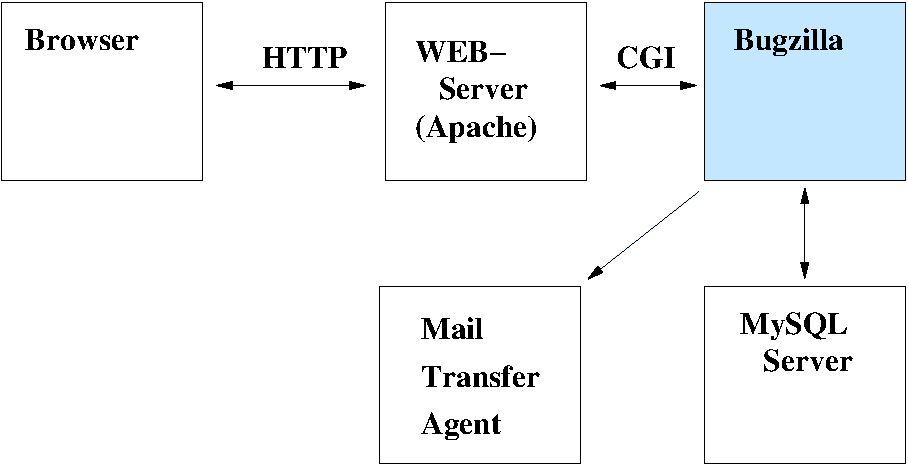
\includegraphics[width=0.56\linewidth]{config-management/xfig/bugzilla}
\end{center}
Bugzilla bietet:

\begin{minipage}{0.48\linewidth}
\begin{itemize}
\item vielfältige Suchmöglichkeiten:
  \begin{itemize}
  \item Welche Probleme sind bekannt, werden bearbeitet, sind behoben?
  \item Welche Releases sind davon betroffen?
  \item Wer ist für das Problem zuständig?
  \item Wie lautet die Problemlösung?
  \end{itemize}
\end{itemize}
\end{minipage}\hfill
\begin{minipage}{0.48\linewidth}
\begin{itemize}
\item vollständige Dokumentationen der Modifikationen (Reports, Grafiken),
\item konfigurierbare Benachrichtigungen bei \"Anderungen,
\item unterschiedliche Schnittstellen: E-Mail, Web, XML, Konsole.
\end{itemize}
\end{minipage}
\begin{figure}[H]
\centering
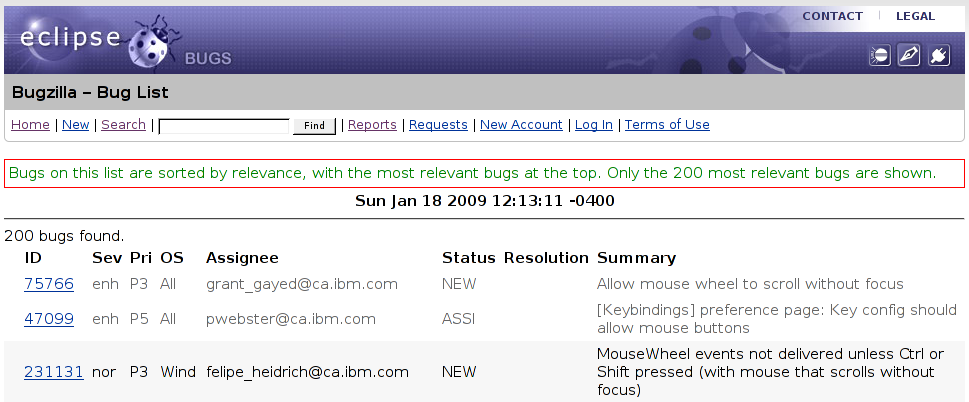
\includegraphics[width=0.85\linewidth]{config-management/bugzilla-buglist1}
\caption{Anzeige der Bug-Liste}
\end{figure}
%---------------------------------------------------------------
\newpage
\ifslides
\begin{center}
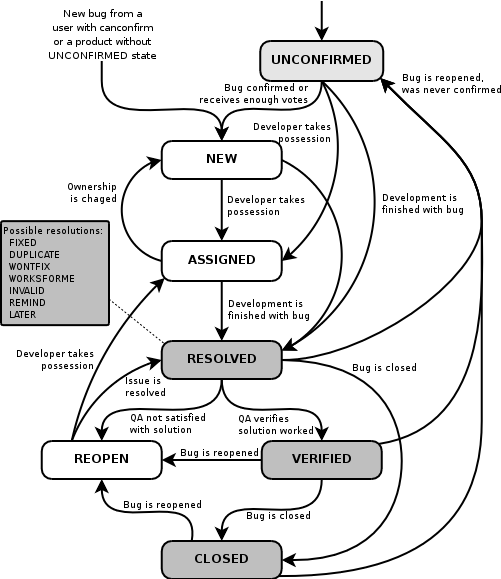
\includegraphics[width= 0.6\linewidth]{config-management/bzLifecycle}
\end{center}
\else
\subsection{Zustandsmodell}
\begin{figure}[H]
\caption{Lifecycle of a Bug}
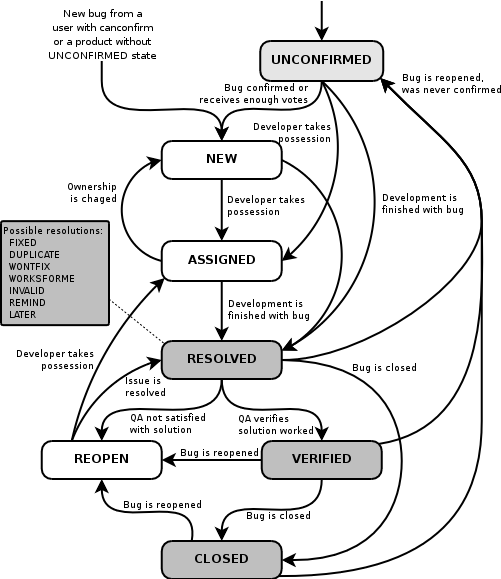
\includegraphics[width= \linewidth]{config-management/bzLifecycle}
\end{figure}
\fi
\newpage
\subsection{Aufbau einer Problemmeldung:}
\ifslides
\else
%Aufbau einer Problemmeldung:\\[2ex]
\fi
\ifslides
{\small
\fi
\begin{tabular}{lp{9.5cm}}
\hline
Product und Component & Ein Produkt kann aus mehreren Komponenten bestehen\\
Status & Zustand der Problemmeldung: UNCONFIRMED, NEW, ASSIGNED, REOPENED,
RESOLVED, VERIFIED, CLOSED\\
Resolution & Behebung: FIXED, INVALID, WONTFIX, LATER, REMIND, DUPLICATE,
WORKSFORME, MOVED\\
Assigned to & die für die Behebung zuständige Person\\
URL & ein mit diesem Problem verknüpfter URL (falls vorhanden)\\
Summary & Zusammenfassung\\
Whiteboard & Beschreibung des Problems\\
Keywords & wichtige Schlüsselbezeichner\\
\ifslides
\end{tabular}
}
\newpage
{\small
\begin{tabular}{lp{9.5cm}}
\fi
Platform und OS & Rechnertyp und Betriebssystem\\
Version & Versionsnummer (Release) des betreffenden Produktes/der Komponente\\
Priority & zugewiesene Priorität: P1 - P5\\
Severity & Auswirkung: blocker, critical, major, normal, minor, trivial,
enhancement\\
Target & voraussichtlicher Release, mit dem das Problem behoben sein wird\\
Reporter & Person, die das Problem gemeldet hat\\
CC & Personen, die bei \"Anderungen des Problemzustandes benachrichtigt
werden\\
Attachments & beiliegende Dateien\\
Dependencies & Abhängigkeiten\\
%%Votes & \\
Comments & Kommentare\\
\hline
\end{tabular}
\ifslides
}
\newpage
\fi
\subsection{Suchen von Bugs mit Bugzilla}
\ifslides
\begin{center}
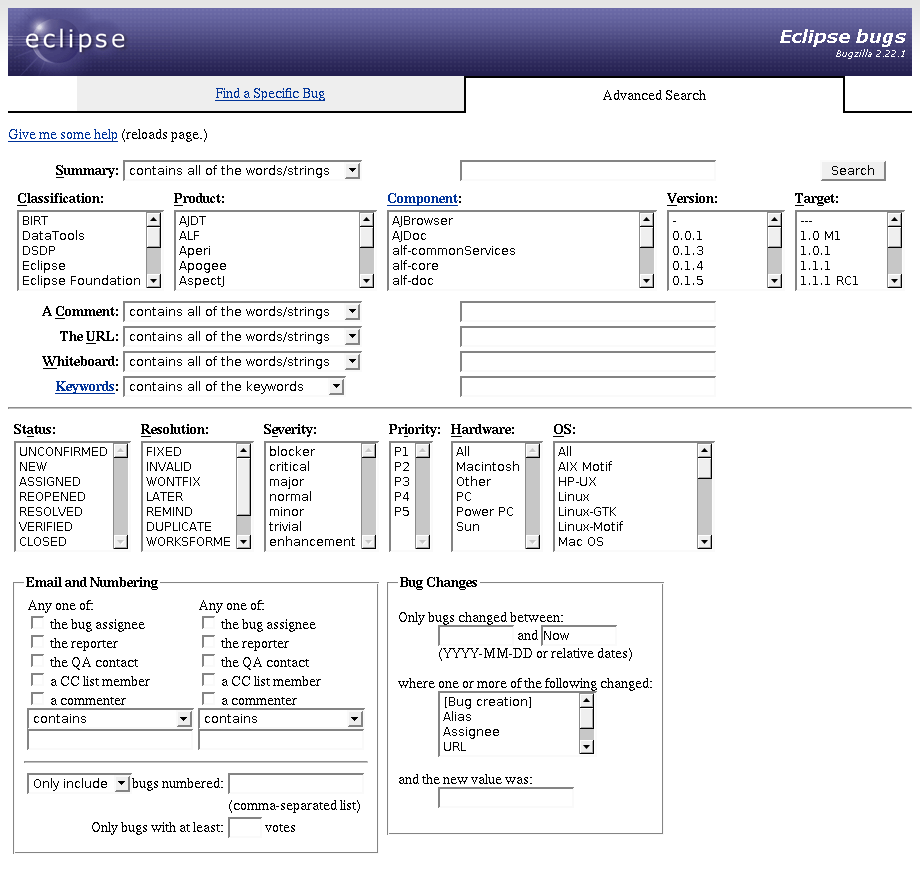
\includegraphics[width=0.6\linewidth]{config-management/bugzilla-search}
\end{center}
\else
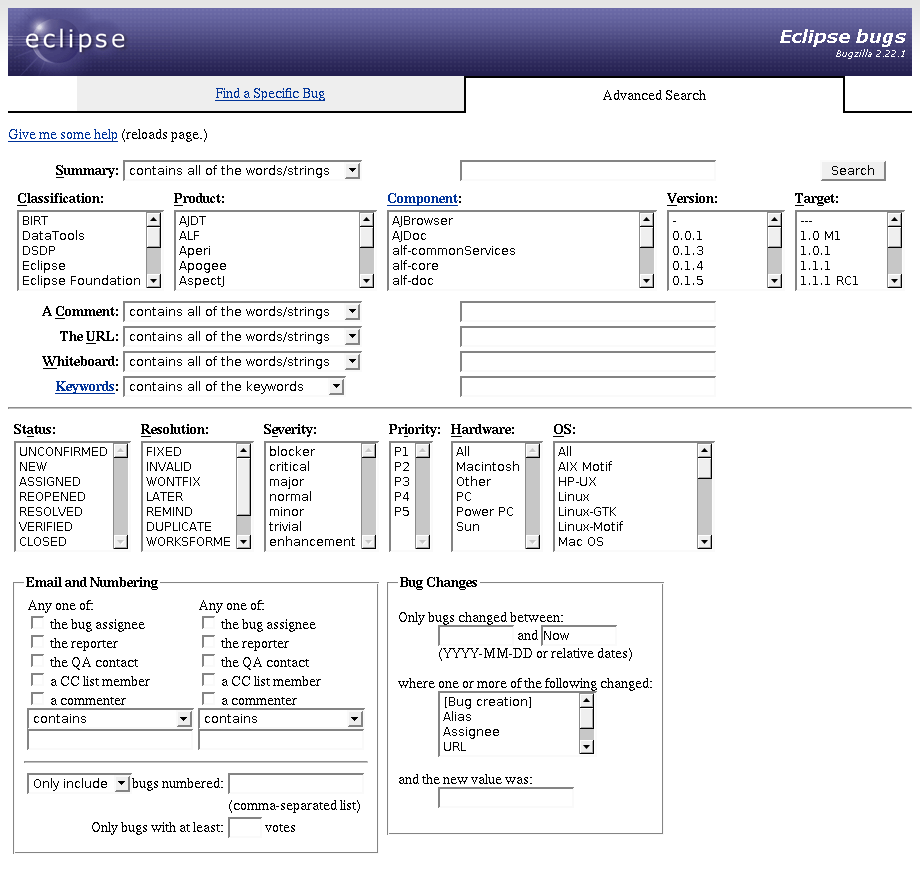
\includegraphics[width=\linewidth]{config-management/bugzilla-search}
\fi
%\newpage
%\subsection{Installation und Konfiguration von Bugzilla}
%Bugzilla kann grundsätzlich auf Mac, Windows und Unix/Linux-Systemen betrieben
%werden. Am einfachsten ist die Installation auf Linux (Details siehe
%Dokumentation):
%\begin{enumerate}
%\item Man installiert, falls nicht bereits vorhanden, Perl, Apache und MySQL.
%\item Man lädt eine aktuelle Bugzilla-Version herunter (2.22) und entpackt
%  sie in ein lokales (Web-) Verzeichnis
%  (z.B. /srv/www/htdocs/bugzilla-2.22). Der Web-Server-User (\verb+wwwrun+)
%  soll Schreibrechte in diesem Verzeichnis haben.
%\item Man installiert allenfalls zusätzlich benötigte
%  Perl-Module:
%  \begin{lstlisting}[language=ksh]
%    checksetup.pl --check-modules
%    perl -MCPAN -e 'install "<modulename>"'
%  \end{lstlisting}
%\item Man installiert einen MTA (sendmail, postfix, exim \ldots), der bei
%  Systemstart gestartet wird.
%\item Man konfiguriert Bugzilla:
%  \begin{enumerate}
%  \item Das Benutzerpasswort für den Datenbank-Benutzer \verb+bugs+.
%\ifslides
%\else
%  (Datei:\verb+localconfig+).
%\fi
%\item Verschiedene MySQL-Parameter: die maximal zulässige Grösse der
%  Attachments,
%  die minimale Wortlänge für die Index-Suche, die maximale Tabellengrösse.
%\item Man legt den Datenbank-Benutzer \verb+bugs+ an und gibt ihm die nötigen
%  Berechtigungen.
%\item Man führt das Skript \verb+checksetup.pl+ aus, welches die Tabellen
%  erzeugt und nach Bedarf weitere Administratoren anlegt.
%  \end{enumerate}
%\item Man konfiguriert den Web-Server, so dass CGI-Skripte im
%  Bugzilla-Verzeichnis ausgeführt werden können (File \verb+httpd.conf+).
%\end{enumerate}
%Bugzilla bietet eine Vielzahl von Konfigurationsmöglichkeiten. Zum Beispiel
%können auf der Basis von Benutzergruppen die Rechte für die Anzeige, das
%Erfassen und Ändern von Einträgen produkt-spezifisch zugeteilt werden.

%\newpage
%\input{mantis}
%\newpage
% http://gushieblog.blogspot.com/2006/11/trac.html
% http://trac-hacks.org/wiki/GitPlugin
%
\section{Trac}
\begin{minipage}{0.55\linewidth}
Trac ist ein erweiterbares Bug-Tracking-Werkzeug mit einer einfachen
Projekt-Management-Funktionalität.
Zusätzlich bietet das von der Firma Edgewood ebenfalls in
Open-Source-Lizenz entwickelte Tool
ein Wiki-System sowie eine Schnittstelle zu verschiedenen Versionsverwaltung-Systemen
(ua. Subversion und Git). Trac basiert auf der Scriptsprache Python und kann
an unterschiedliche Datenbanken angepasst werden.
\end{minipage}
\hfill
\begin{minipage}{0.4\linewidth}

\includegraphics[width=\linewidth]{config-management/trac_diagram}
\end{minipage}
%
\ifslides
\begin{center}
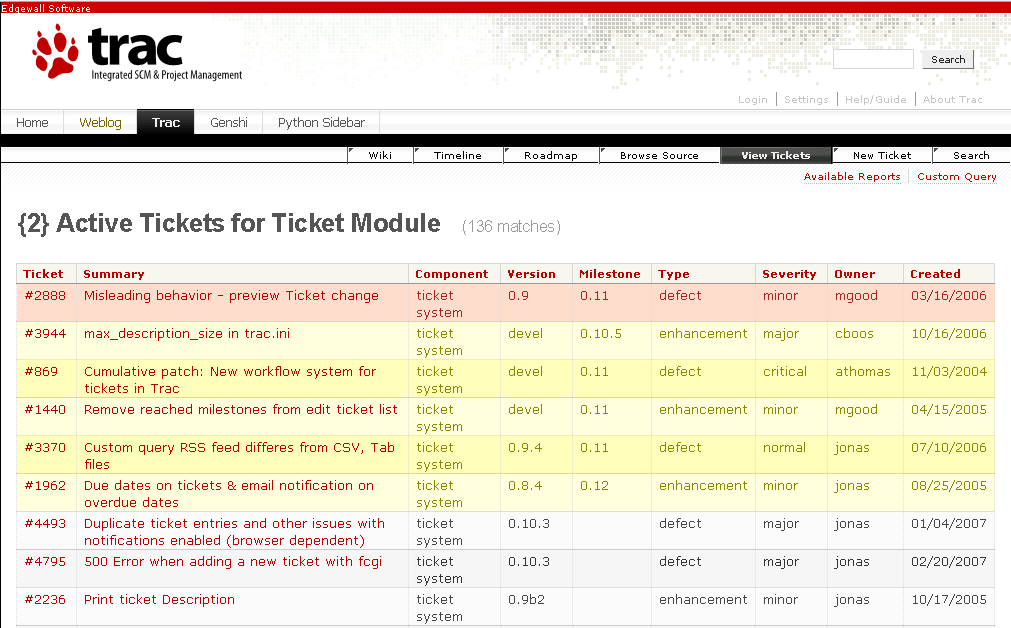
\includegraphics[width=\linewidth]{config-management/trac-ticketlist}
\end{center}
\else
\begin{figure}[H]
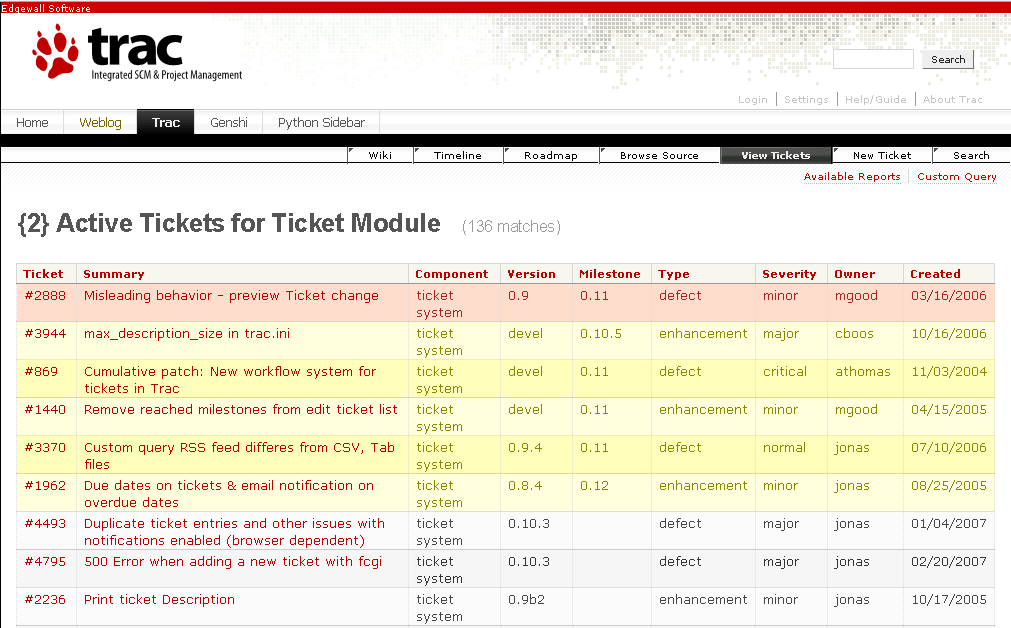
\includegraphics[width=\linewidth]{config-management/trac-ticketlist}
\caption{Anzeige der Ticket-Liste bei Trac}
\end{figure}
\fi
\ifslides
\begin{figure}[H]
\begin{center}
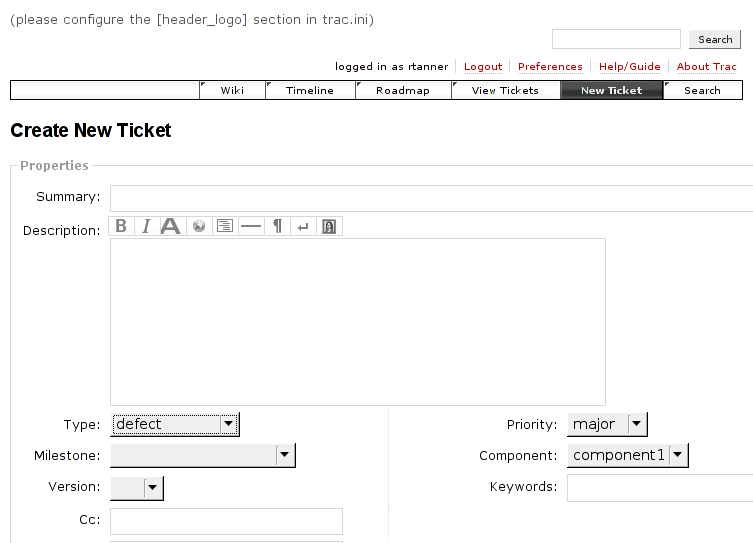
\includegraphics[width=0.7\linewidth]{config-management/trac-newticket}
\caption{Erfassen eines Tickets bei Trac}
\end{center}
\end{figure}
\else
\begin{figure}[H]
\begin{center}
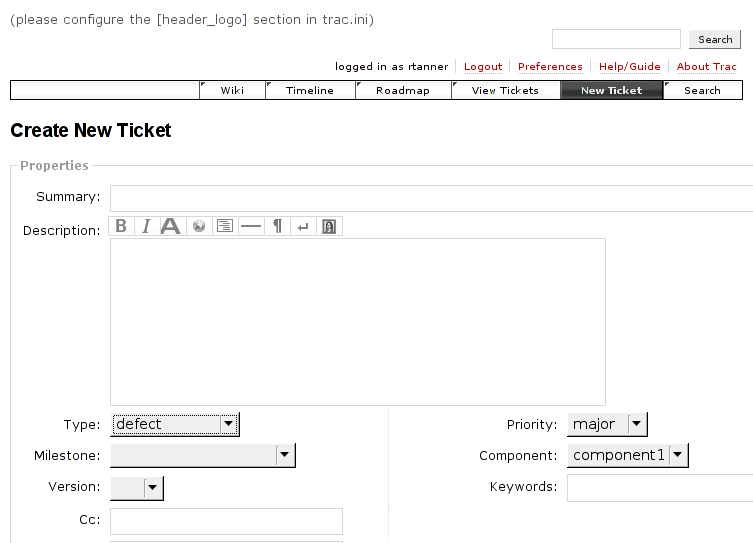
\includegraphics[width=0.8\linewidth]{config-management/trac-newticket}
\caption{Erfassen eines Tickets bei Trac}
\end{center}
\end{figure}
\fi
%
\ifslides
\begin{figure}[H]
\begin{center}
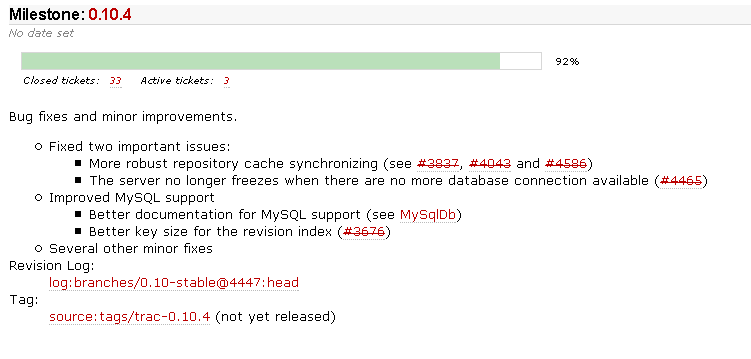
\includegraphics[width=\linewidth]{config-management/trac-roadmap}
\caption{Roadmap bei Trac}
\end{center}
\end{figure}
\else
\begin{figure}[H]
\begin{center}
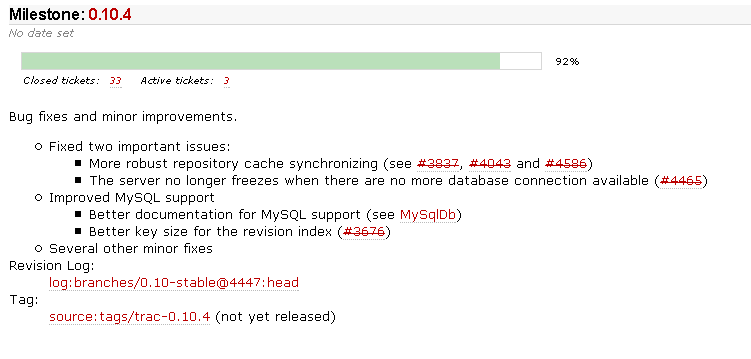
\includegraphics[width=0.8\linewidth]{config-management/trac-roadmap}
\caption{Roadmap bei Trac}
\end{center}
\end{figure}
\fi
\subsection{Workflow}
Beim Arbeiten mit Trac muss einer konfigurierten Abfolge von Schritten,
einem sogenannten Workflow, der vom Zustand
des Tickets gesteuert wird, gefolgt werden. Die Workflow-Regeln können im
Konfigurations-File trac.ini festgelegt werden. Bei der
Installation von Trac wird der in Abbildung \ref{fig:trac-workflow}
dargestellte Workflow eingestellt.
\begin{figure}[H]
  \centering
  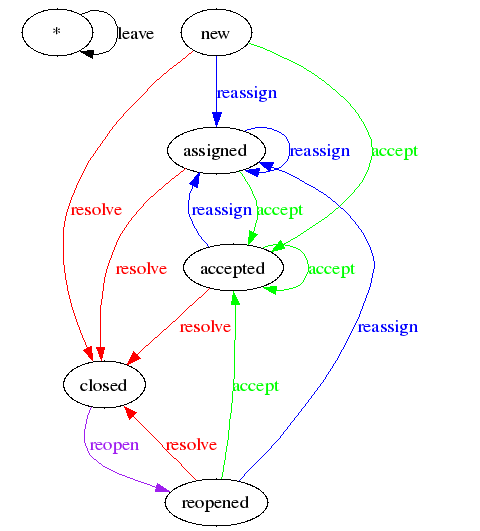
\includegraphics[width=0.5\linewidth]{config-management/trac-workflow}
  \caption{Default-Workflow}
  \label{fig:trac-workflow}
\end{figure}
%
\paragraph{\underline{1. Erfassen eines Tickets}}
Ein angemeldeter Benutzer mit der zugeteilten Berechtigung
\verb+TICKET_CREATE+ kann ein neues Ticket erfassen.
Ein Ticket kann eine Fehlermeldung, ein
  Änderungsvorschlag, eine Idee für eine Erweiterung sein.
  Es müssen dabei die folgenden Informationen
  eingeben werden:
  \begin{description}
    \item [Summary] eine Kurzbeschreibung des Inhalts
    \item [Description] die ausführliche Beschreibung
    \item[Type] der Typ des Tickets:
      \begin{itemize}
      \item defect: ein Bug, eine Störung, etwas was nicht so
        funktioniert, wie es
        erwartet wird oder dokumentiert ist,
      \item enhancement: eine Erweiterung, Verbesserung des
        bestehenden Systems,
      \item Task: ein Auftrag, der erledigt werden muss/sollte
      \end{itemize}
      Die Liste kann vom Administrator geändert und ergänzt werden.
\newslide
      \item [Priority:] die Auswirkung resp. Dringlichkeit
        \begin{center}
        \begin{tabular}{llll}
          Priority & Weiterarbeit & Verbesserung & Behebung/Umsetzung\\
          \hline
         {\bfseries blocker} &  nicht möglich & unverzichtbar & unverzüglich \\
         {\bfseries critical} & erheblich eingeschränkt & bedeutend & möglichst bald\\
       {\bfseries major} & eingeschränkt & wichtig & innerhalb kurzer Zeit\\
        {\bfseries minor} & leicht eingeschränkt & geringfügig & bald \\
        {\bfseries trivial} & marginal eingeschränkt & kosmetisch & offen \\
      \end{tabular}
    \end{center}
\newslide
  \item[Milestone] der Release, bei welchem das Problem behoben sein
    sollte,
  \item[Component] die betroffene Komponente (Teilsystem),
  \item[Version] die betroffene Version des verwendeten Systems (nur
    bei defects),
  \item[CC] E-Mail-Adressen und/oder Benutzer, die bei Änderungen
    benachrichtigt werden sollen,
   \item[Estimated Number of Hours] der geschätzte Aufwand in Stunden,
   \item[Add hours to ticket] der neu geleistete Aufwand in Stunden,
   \item[Assign to] die für die Behebung zuständige Person,
   \item[I have files to attach] wenn Dateien (Screenshots,
     Log-Dateien, Patches\ldots) hinzugefügt werden sollen.
  \end{description}
%
\newslide
\paragraph{\underline{2. Bearbeiten eines Tickets}}
Nachdem ein Ticket erfasst ist, kann es von jedem Benutzer mit der zugeteilten
Berechtigung \verb+TICKET_MODIFY+ modifiziert werden. Alle Änderungen
werden mit Datum und Benutzername aufgezeichnet.
%und können mit den
%Menupunkten ''View Tickets'' oder ''Timeline'' angezeigt werden.

Tickets können auf unterschiedliche Art gesucht und angezeigt werden:
\begin{itemize}
\item Search: Eingabe eines Such-Textes
\item View Tickets: Ausgabe einer sortierten Ticket-Liste nach unterschiedlichen
  Filter- und Gruppierkriterieren:
  \begin{itemize}
  \item active: alle Tickets, die noch nicht abgeschlossen sind,
  \item active by version: dito, gruppiert nach Version,
  \item active tickets by milestone: dito, gruppiert nach Milestone,
  \item accepted by owner: alle Tickets, die akzeptiert aber noch
    nicht abgeschlossen sind, gruppiert nach Besitzer,
  \item all by milestone: alle Tickets gruppiert nach Milestone
  \item my tickets: alle Tickets, die dem Benutzer zugewiesen sind
  \end{itemize}
\end{itemize}
\newslide
Wenn ein Ticket erfasst worden ist, erhält es den Zustand ''New''. Es
muss innerhalb einer festzulegenden Periode geprüft, fehlende oder
inkorrekte Einträge müssen korrigiert oder ergänzt und einem
Bearbeiter zugewiesen, resp. von einem Bearbeiter akzeptiert
werden. Insbesondere müssen vor einer Zuweisung die folgenden Werte
korrekt gesetzt werden:
\begin{itemize}
  \item Milestone
  \item Version (nur bei einem defect)
\end{itemize}
Ein zugewiesenes Ticket muss von einem Bearbeiter akzeptiert
werden. Er setzt dabei den geschätzten Aufwand im Textfeld ''estimated
number of hours''.
%
\newslide
\paragraph{\underline{3. Abschliessen eines Tickets}}
Das Ticket wird mit ''resolve as'' und der Angabe des geleisteten Aufwands
geschlossen. Dabei muss eines der folgenden
Attribute gewählt werden:
\begin{description}
\item[fixed] das Problem ist behoben resp. die Verbesserung ist
  implementiert, getestet und eingecheckt.
\item[invalid] das Ticket ist ungültig, weil es entweder einen
  Sachverhalt beschreibt, der beabsichtigt ist, oder weil das Problem
  ein anderes System betrifft.
\item[wontfix] das beschriebene Problem kann aus technischen oder
  ökonomischen Gründen nicht behoben werden.
\item[duplicate] das Problem ist bereits von einem anderen Ticket beschrieben.
\item[worksforme] das Problem kann nicht reproduziert werden.
\end{description}
Der jeweilige Entscheid muss im Textfeld ''Add/Change'' begründet werden.

Ein bereits geschlossenes Ticket kann mit ''reopen' wieder geöffnet werden.
%
\newpage
\section{Gitlab: Issues}
\ifslides
\begin{picture}(0,0)
\put(250,22){
  
\includegraphics[width=4cm]{config-management/gitlab-logo}
}
\end{picture}
\else
\begin{picture}(0,0)
\put(280,17){
  
\includegraphics[width=3.7cm]{config-management/gitlab-logo}
}
\end{picture}
\fi
The GitLab issue tracker is an advanced tool for collaboratively
developing ideas, solving problems, and planning work.
\begin{figure}[H]
  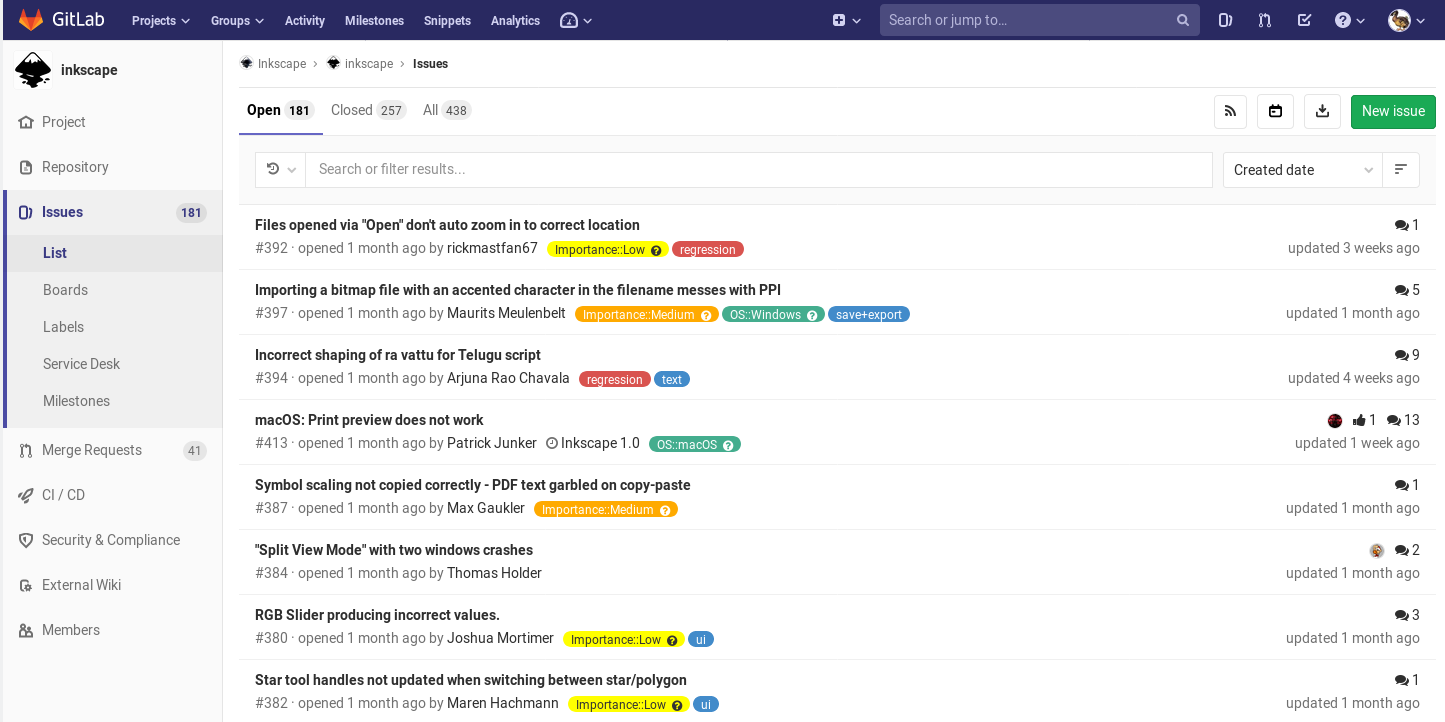
\includegraphics[width=\linewidth]{config-management/gitlab-issues}
  \caption{Gitlab Issue Example}
\end{figure}
\begin{figure}[H]
  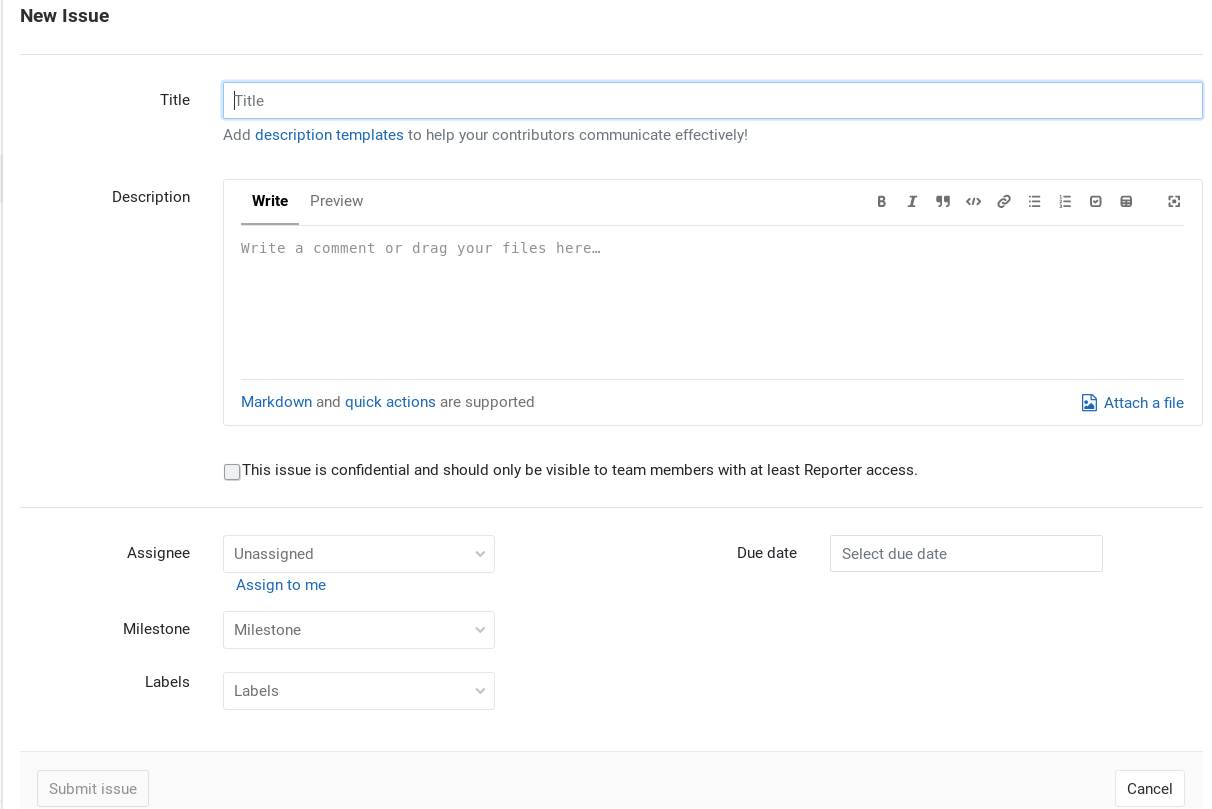
\includegraphics[width=\linewidth]{config-management/gitlab-new-issue}
  \caption{Gitlab New Issue}
\end{figure}
Concepts:
\begin{description}
\item[Labels]: categorize issues or merge requests using descriptive titles like bug, feature request, or docs
\item[Issue Boards]: groups issues in lists that correspond to their assigned labels,
  visualizing issues designed as cards throughout those lists.
\item[Milestones]: group issues and merge requests with an optional start date and an optional due date.
\end{description}

\newpage
\section{JIRA}
\ifslides
\begin{picture}(0,0)
\put(270,22){

\includegraphics[width=2.5cm]{config-management/jira-logo}
}
\else
\begin{picture}(0,0)
\put(300,22){

\includegraphics[width=2.5cm]{config-management/jira-logo}
}
\fi
\end{picture}
JIRA ist ein Problemverwaltungsystem, oder vielleicht zutreffender,
ein kommerzielles, populäres, umfassendes, konfigurierbares Pendenzen- und
Projektverwaltungssystem
(Issue Tracking and Project Management) auf Java-EE-Basis.
%welches für Non-Profit-Organisationen und Open-Source-Projekte
%kostenfrei eingesetzt werden kann.
\ifslides
\begin{figure}[H]
\begin{center}
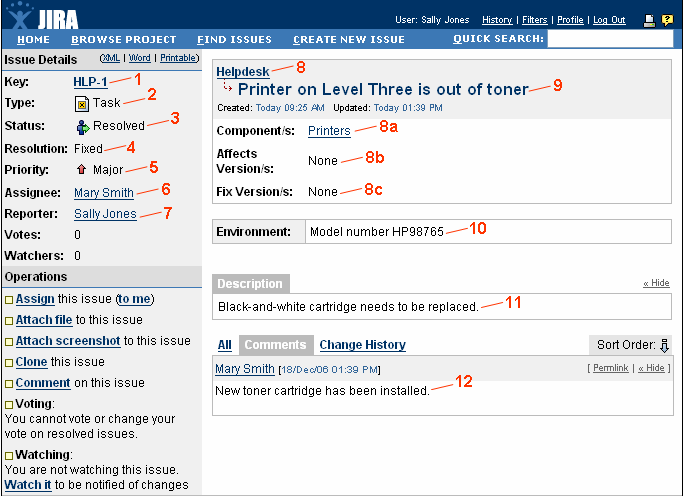
\includegraphics[width=0.9\linewidth]{config-management/jira-issue-overview}
\end{center}
\caption{Anzeigen einer Pendenz bei JIRA}
\end{figure}
\else
\begin{figure}[H]
\begin{center}
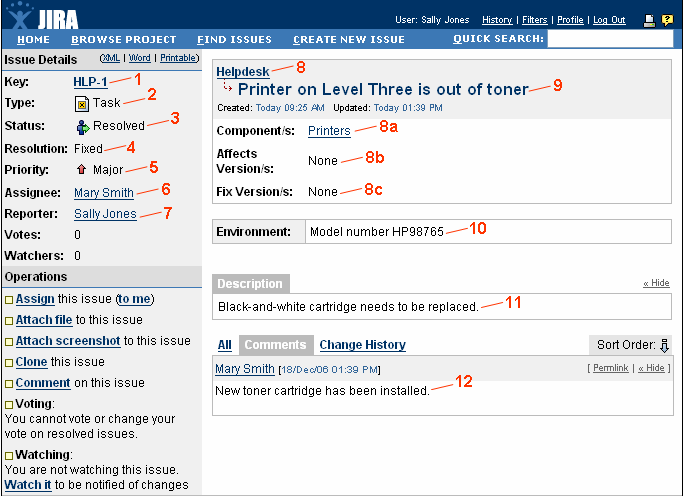
\includegraphics[width=\linewidth]{config-management/jira-issue-overview}
\end{center}
\caption{Anzeigen einer Pendenz bei JIRA}
\end{figure}
\fi
%
\begin{enumerate}
\item {\bfseries Key}: ein eindeutiger Kennzeichner.
\item {\bfseries Type}: Bug, Improvement, New feature, Task, Custom issue
\item {\bfseries Status}: der Zustand, den die Pendenz gegenwärtig einnimmt:
   Open, In Progress, Resolved, Reopened, Closed.
\item {\bfseries Resolution}: ob und wie die Pendenz erledigt ist:
  Fixed, Won't Fix, Duplicate, Incomplete, Cannot Reproduce.
\item {\bfseries Priority}: die Wichtigkeit in Bezug zu anderen Pendenzen:
   Blocker, Critical, Major, Minor, Trivial.
\item {\bfseries Assignee}: die Person, welcher die Pendenz zugewiesen ist.
\item {\bfseries Reporter}: die Person, die die Pendenz erfasst hat.
\newslide
\item {\bfseries Project}:  das zugeordnete Projekt
\begin{enumerate}
  \item Component(s): die betroffenen Projekt-Komponenten
  \item Affects Version(s): die betroffenen Versionen
  \item Fix Version(s)*: die Projekt-Versionen, bei welchen das
      Problem behoben ist (oder sein wird)
  \end{enumerate}
\item {\bfseries Summary}: eine Kurzbeschreibung
\item {\bfseries Environment}*
  die betroffene Hardware oder Software-Umgebung
\item {\bfseries Description} die detaillierte, (nachvollziehbare!) Beschreibung
\item {\bfseries Comments}: allfällige Kommentare der Bearbeiter
  \end{enumerate}
%
\begin{figure}[H]
\begin{center}
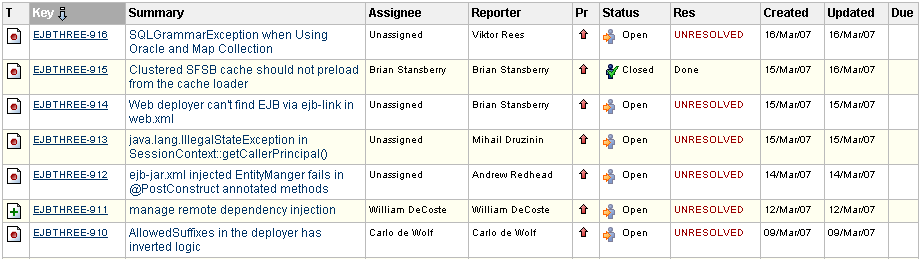
\includegraphics[width=\linewidth]{config-management/jira-issue-list}
\end{center}
\caption{Eine Pendenzenliste bei JIRA}
\end{figure}
%
\begin{figure}[H]
\begin{center}
\ifslides
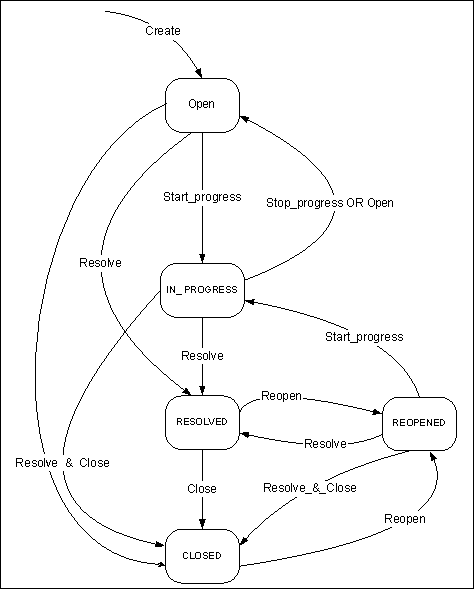
\includegraphics[width=0.4\linewidth]{config-management/jira-workflow-statediagram}
\else
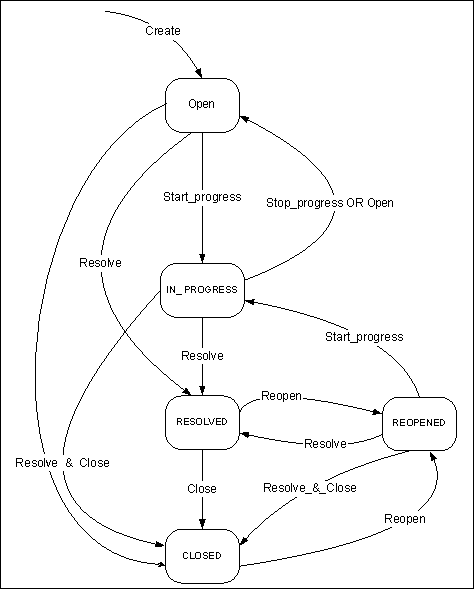
\includegraphics[width=0.6\linewidth]{config-management/jira-workflow-statediagram}
\fi
\end{center}
\caption{Default-Workflow bei JIRA}
\end{figure}
%

%
\newpage
\section{Exercises}
\begin{enumerate}
\item Untersuchen und vergleichen Sie die Charakteristiken
  verschiedener Projekte, die Bugzilla, Mantis, JIRA oder
  Trac einsetzen. Welchen betrieblichen Nutzen haben
  diese Bug-Tracking-Systeme?
  Welche Reporting-Möglichkeiten gibt es und welche
  geschäftsrelevanten Schlüsse lassen sich daraus ziehen?
\item Führen Sie mit Trac oder Gitlab für das Histogram-Projekt
die folgenden Schritte durch:
\begin{enumerate}
\item Erstellen Sie die Meilensteine ``rel-0.0'', ``rel-0.1'' und ``rel-0.2''
\item Erstellen Sie die Tickets/Issues
  \begin{itemize}
  \item Einrichten des Projektes,
  \item Erstellen einer ausführbaren JAR-Datei mit Ant
  \item Erstellen einer ausführbaren JAR-Datei mit Maven
  \end{itemize}
 und weisen Sie die Tickets jeweils einem Meilenstein zu.
\end{enumerate}
\end{enumerate}
%{\bfseries Bewertung:} Vollständigkeit, Korrektheit, Nachvollziehbarkeit
%
\newslide
\section{Software and further Informationa}
\begin{itemize}
\item Bugzilla: \href{https://www.bugzilla.org}{www.bugzilla.org}
%\item Bugzilla Test Server: \href{http://landfill.bugzilla.org}
%                                 {landfill.bugzilla.org}
\item Trac: Integrated SCM and Project Management
% an enhanced wiki and issue tracking system for software
%  development projects.
  \href{https://www.edgewall.org/trac}{www.edgewall.org/trac}
  \item Gitlab: \href{https://docs.gitlab.com/ee/README.html}{docs.gitlab.com/ee/README.html}
\item Mantis BT: \href{https://www.mantisbt.org}
  {www.mantisbt.org}
\item Redmine \href{https://www.redmine.org}{www.redmine.org}
\item JIRA: \href{https://www.atlassian.com/software/jira}
  {www.atlassian.com/software/jira}
\end{itemize}
\newpage
